\documentclass[11pt, a4paper]{article}

%% Packages
\usepackage{amsmath}
\usepackage{amsfonts,amsthm,amssymb,enumerate}
\usepackage{pgf,tikz}
\usepackage{graphicx}
\graphicspath{{./figures/}}
\usepackage[hidelinks]{hyperref}

%% Page style
\setlength{\parindent}{0pt}
\setlength\parskip{.7em plus 0.1em minus 0.2em}
\usepackage{fancyhdr}
\pagestyle{fancy}
\fancyhf{}
\renewcommand{\footrulewidth}{0.4pt}
\cfoot{Page \thepage\ of \pageref{lastpage}}
\rhead{Draft \textit{\number\day/\number\month/\number\year}}
\lhead{\leftmark}
\fancyheadoffset{0cm}

\usepackage[headsep=.5cm,headheight=14.5pt,margin=3cm]{geometry}
%\usepackage{showframe}

%% Shortcuts
\newcommand{\CC}{\mathbb{C}}
\newcommand{\RR}{\mathbb{R}}
\newcommand{\NN}{\mathbb{N}}
\newcommand{\QQ}{\mathbb{Q}}
\newcommand{\ZZ}{\mathbb{Z}}
\newcommand{\FF}{\mathbb{F}}
\newcommand{\PP}{\mathbb{P}}
\newcommand{\KK}{\mathbb{K}}
\newcommand{\OO}{\mathcal{O}}
\newcommand{\inv}{^{-1}}
\renewcommand{\epsilon}{\varepsilon}
\renewcommand{\phi}{\varphi}

%% Theorems
\newtheoremstyle{break}
{\topsep}{\topsep}%
{}{}%
{\bfseries}{}%
{\newline}{}%

\theoremstyle{break}
\newtheorem{thm}{Theorem}[section]
\newtheorem{cor}[thm]{Corollary}
\newtheorem{prop}[thm]{Proposition}
\newtheorem{propdefn}[thm]{Proposition/Definition}
\newtheorem{lemdefn}[thm]{Lemma/Definition}
\newtheorem{eg}[thm]{Example}
\newtheorem{ex}[thm]{Exercise}
\newtheorem{lem}[thm]{Lemma}
\newtheorem{note}[thm]{Note}
\newtheorem{defn}[thm]{Definition}
\newtheorem{rmk}[thm]{Remark}
\newtheorem{re}[thm]{Results}
\newtheorem{code}[thm]{Code}
\newenvironment{prf}[1][\proofname]{%
	\begin{proof}[#1]$ $\par\nobreak\ignorespaces
	}{%
	\end{proof}
}

%% Code
\usepackage{listings}
\lstset{language=Python,upquote=true, 
	numbers=left, stepnumber=1, 
	basicstyle=\small\ttfamily,columns=fullflexible,tabsize=5, xleftmargin=.25in, 	showstringspaces=false,breaklines=true,keepspaces}

%% Magic
\makeatletter
\newcommand*{\perm}[1]{\text{$(\@for\tmp:=#1\do{{\tmp}\;}\hspace{-.277em})$}}%permutation
\makeatother
\makeatletter
\newcommand*{\permcom}[1]{\text{$(#1)$}}%permutation
\makeatother
\newcommand*{\ideal}[1]{\text{$\langle#1\rangle$}}%ideal
\newcommand*{\Ideal}[1]{\text{$\left\langle#1\right\rangle$}}%ideal
\def\matrixtwooneHelp(#1,#2){\begin{pmatrix}#1\\#2\end{pmatrix}}%matrix
\def\matrixtwoHelp(#1,#2,#3,#4){\begin{pmatrix}#1&#2\\#3&#4\end{pmatrix}}%matrix
\def\matrixthreeHelp(#1,#2,#3,#4,#5,#6,#7,#8,#9){\begin{pmatrix}#1&#2&#3\\#4&#5&#6\\#7&#8&#9 \end{pmatrix}}%matrix
\newcommand*{\matrixtwo}[1]{\matrixtwoHelp(#1)}
\newcommand*{\matrixtwoone}[1]{\matrixtwooneHelp(#1)}
\newcommand*{\matrixthree}[1]{\matrixthreeHelp(#1)}
\newcommand*{\size}[1]{|#1|}%size of group
\newcommand*{\Size}[1]{{\left|#1\right|}}%big size
\newcommand*{\ind}[2]{|#1:#2|}
\newcommand*{\set}[1]{\{#1\}}%set 
\newcommand*{\Set}[1]{\left\{#1\right\}}%set 
\newcommand*{\paren}[1]{(#1)}%set 
\newcommand*{\Paren}[1]{\left(#1\right)}%set 
\newcommand{\cross}{\times}
\newcommand{\rcross}{\rtimes}
\newcommand{\lcross}{\ltimes}
\newcommand{\id}{\mathsf{id}}


%% Specific commands
\newcommand{\ve}{\mathbf} % Vectors
\newcommand{\dt}{\Delta t}
\newcommand{\dx}{\Delta x}
\newcommand{\der}[2]{\frac{\partial #1}{\partial #2}}
\newcommand{\pder}[3][2]{\frac{\partial^#1 #2}{\partial #3^#1}}
\newcommand{\dder}[2]{\frac{d #1}{d #2}}
\newcommand{\ddder}[3][2]{\frac{d^#1 #2}{d #3^#1}}
\newcommand{\eval}[1]{\big\rvert_{#1}}
\newcommand{\Eval}[1]{\bigg\rvert_{#1}}
\newcommand{\dd}{\ \mathrm{d}}
\begin{document}
\begin{center}
{\LARGE Numerical Methods}\\
{\large Compiled by Tristan Pang}\\
{\the\month/\the\year}
\end{center}
These notes are based on the Oxford Numerical Methods course taught by David Marshall (2023 for the NERC DTP) with additional information from LeVeque \cite{leveque_finite_2007}.

These are rough notes only. A polished version may or may not be completed. Please direct all typos to me. The \href{https://github.com/tristanpang/numerical-methods-notes}{GitHub repo}\footnote{https://github.com/tristanpang/numerical-methods-notes} contains \LaTeX\ source, Python scripts for figures, and other useful Python things.

\tableofcontents



\section{Root finding}
Consider a sufficiently smooth function $f(x)$. If $f$ is a quadratic polynomial, we may find the zeros of $f$ using the quadratic formula, but for degrees 5 or larger, there exists no general formula for the zeros (Abel–Ruffini theorem). In general, finding an $x^*$ such that $f(x^*)=0$ cannot be computed exactly. Instead one must employ numerical root finding algorithms. Common methods include the bisection method and Newton's method.

\subsection{Bisection method}
To find a zero $x^*$ of $f$, the bisection method takes two initial guesses $a$ and $b$ such that $a<0$ and $b\geq0$. IVT guarantees a zero between the two guesses. Calculate the midpoint \[c=\frac{a+b}2.\] If $f(c)<0$, replace $a$ with $c$; otherwise replace $b$ with $c$. Continue iterating until convergence is observed as shown in Figure~\ref{fig:bisection}.

\begin{figure}\centering
	\includegraphics[width=0.7\textwidth]{example-image-golden}
	\caption{Bisection method}\label{fig:bisection}
\end{figure}

The error at the first iteration is \begin{align*}
\epsilon_1 &= |c - x^*| \\&= \Size{\frac{a-x^*}{2}+\frac{b-x^*}{2}}\\&= \Bigg|\Size{\frac{a-x^*}{2}}-\Size{\frac{b-x^*}{2}}\Bigg| \\&\leq \Size{\frac{a-x^*}{2}-\frac{b-x^*}{2}}\\
&= \frac{|b-a|}{2}.\end{align*}
Thus, in general \[\epsilon_n = |c-x^*| \leq \frac{|b-a|}{2},\] i.e. the error is at least halved each iteration, and the method converges linearly.
\begin{eg}
The positive zero of the polynomial $f(x)=x^2-2$ can be approximated using bisection with starting guesses $a=1$ and $b=2$. Then $f(1)=-1<0$ and $f(2)=2>0$. It follows (by continuity of $f$) that there is a root in the interval $[1,2]$. Then $f(c)=f(1.5)=0.25>0$. Thus, we replace $b=2$ with $c=1.5$. Continuing yields $1.25, 1.375, 1.4375, \ldots$. Eventually, we get an approximation for  $\sqrt 2$.
\end{eg}

\subsection{Newton's method}
A quicker alternative to bisection is Newton's method (also known as Newton-Raphson). Given an initial guess $x_0$ and a sufficiently nice derivative $f'$, we may estimate a zero $x^*$ of $f$.

Consider the Taylor expansion of $f$ around $x_n$ (see Appendix~\ref{sec:bigO} for the big $O$ notation and Appendix~\ref{sec:taylor} for Taylor): \[f(x)=f(x_n)+f'(x_n)(x-x_n)+O((x-x_n)^2).\] If we suppose that $x_n$ is close to the root $x^*$, the zero of the linear approximation $x_{n+1}$ is a good approximation for $x^*$ \[f(x_{n+1})\approx 0=f(x_n)+(x_{n+1}-x_n)f'(x_n).\] Rearranging, we arrive at the iterative formula for Newton's method \begin{equation}\label{eq:newtonStep} x_{n+1} = x_n-\frac{f(x_n)}{f'(x_n)}.\end{equation} This process is illustrated in Figure~\ref{fig:taylor}.

\begin{figure}\centering
	\includegraphics[width=0.7\textwidth]{example-image-golden}
	\caption{Newton's method}\label{fig:taylor}
\end{figure}

The signed error at iteration $n$ is $\epsilon_n = x_n-x^*$. By considering the quadratic term in the Taylor expansion around $x_n$, we get \begin{align*}f(x^*)&=f(x_n)+f'(x_n)(x^*-x_n)+\frac{f''(x_n)}{2}(x^*-x_n)^2 + O((x^*-x_n)^3)\\
\implies\quad& 0 = f(x_n) + f'(x_n)(x^*-x_n)+\frac{f''(x_n)}{2}\epsilon_n^2 + O(\epsilon_n^3)\\
\implies\quad& -\frac{f(x_n)}{f'(x_n)}=(x^*-x_n)+\frac{f''(x_n)}{2}\epsilon_n^2 + O(\epsilon_n^3)\\
\implies\quad& x_{n+1}-x_n=(x^*-x_n)+\frac{f''(x_n)}{2}\epsilon_n^2 + O(\epsilon_n^3)\\
 \implies\quad&\epsilon_{n+1}=\frac{f''(x_n)}{2}\epsilon_n^2 + O(\epsilon_n^3)
\end{align*}

Thus, as $n\to \infty$, $x_{n}\to x^*$ for a root $x^*$ of $f$. In particular, we have quadratic convergence.

\begin{eg}
The positive zero of the polynomial $f(x)=x^2-2$ can be approximated using Taylor's method with the starting guess $x_0=2$. Differentiating, $f'(x)=2x$. Then we get \begin{align*}
x_1 &= x_0 - \frac{f(x_0)}{f'(x_0)} = 2 - \frac{2^2-2}{4} = 1.5,\\
x_2 &= 1.5 - \frac{1.5^2-2}{3} = 1.41666667,\\
x_3 &= 1.41421569,\\
x_4 &= 1.41421356 \approx\sqrt{2}.
\end{align*}
This converges to $\sqrt{2}$ much faster than the bisection method as seen in Figure~\ref{fig:bisectionVsNewton}.
\begin{figure}\centering
	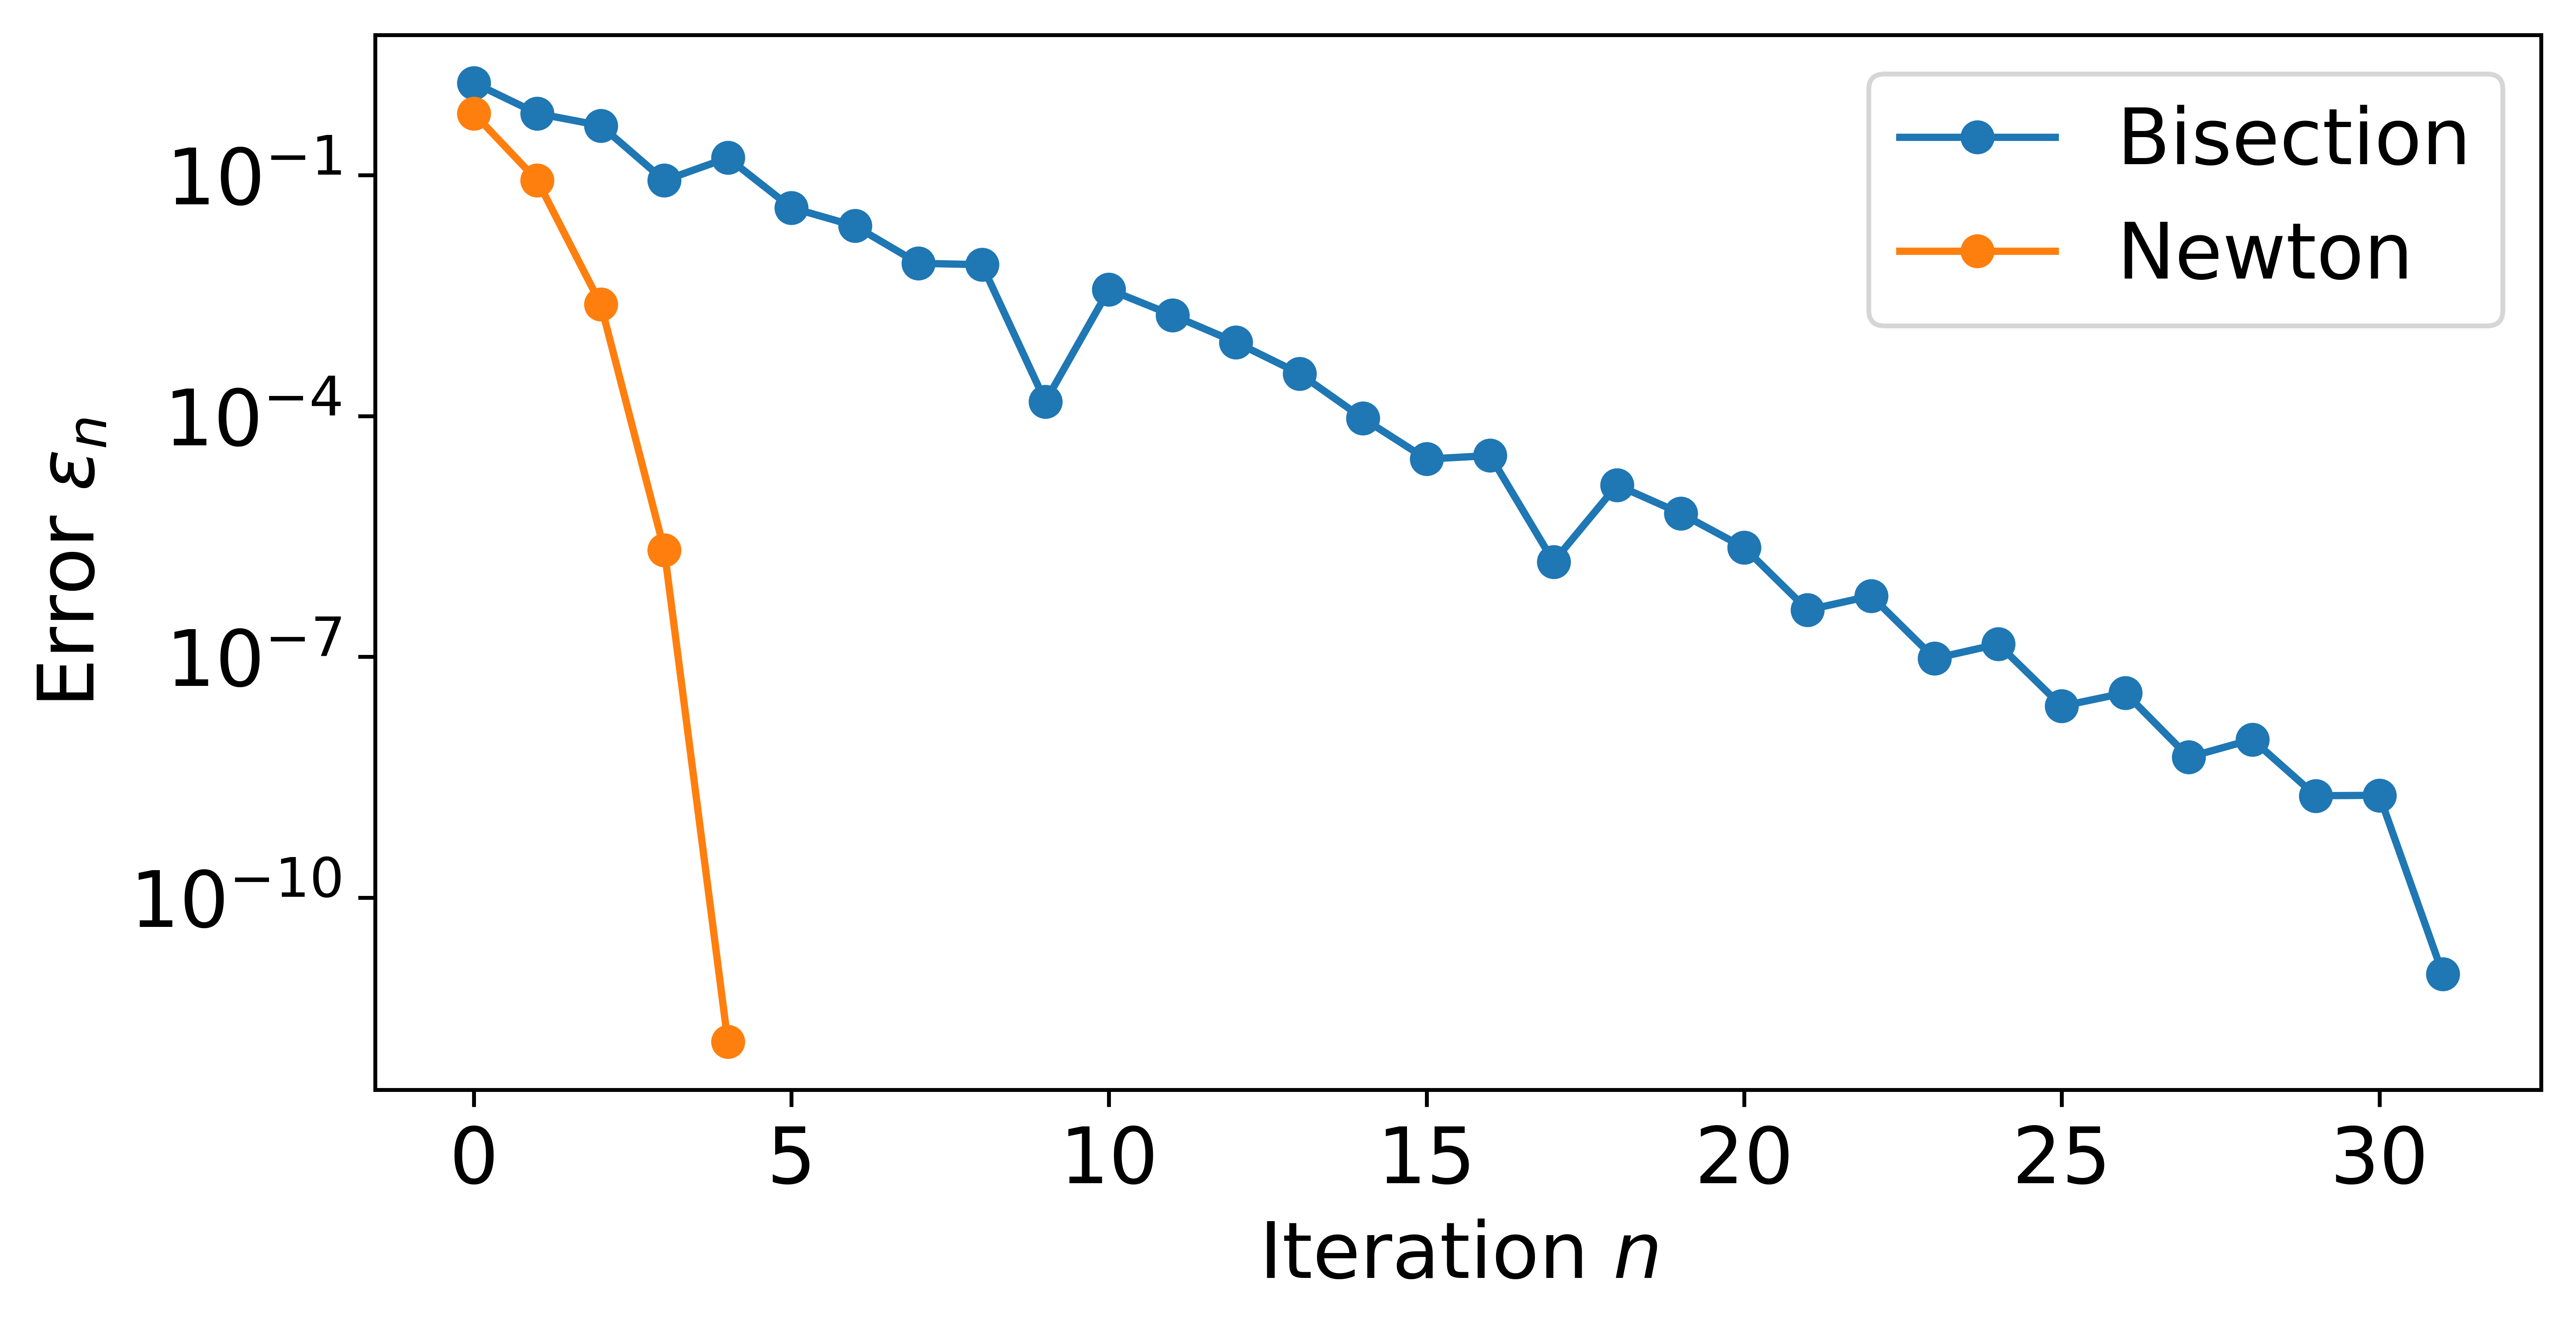
\includegraphics[width=0.7\linewidth]{bisectionVsNewton}
	\caption{Bisection method vs Newton's method for approximating $\sqrt2$}\label{fig:bisectionVsNewton}
\end{figure}
\end{eg}

\begin{ex}
	Observe (in Python or otherwise) that approximating $\sqrt2$ with a bisection guess of $(1, 200)$ and Newton guess of $200$ yields similar log-linear error behaviour for small iteration step~$n$. Show that this is true by looking at Formula~\ref{eq:newtonStep}.
\end{ex}
Warning: if $f'(x_n)=0$, Newton's method will not work (division by zero!) -- pick a new~$x_0$. If the derivative is not well behaved (either not defined or close to zero at many points), then Newton's method may not be appropriate.


\subsection{Higher dimensions}
Consider the system of $m$ equations in $n$ variables $\ve{f}(\ve x)=\ve 0$ given by \[\begin{cases} f_1(x_1,x_2, \ldots, x_n) =0,\\f_2(x_1,x_2,\ldots, x_n)=0, \\\hfil\vdots\\ f_m(x_1,x_2,\ldots,x_n)=0.\end{cases}\]
The iterative step of Newton's method becomes \begin{equation}
	\label{eq:newtonDim}\ve x_{n+1}=\ve x_n-J(\ve x_n)\inv \ve{f}(\ve x_n),
\end{equation} where $J$ is the Jacobian matrix of $\mathbf f$ (an analogue to the derivative) given by $J_{ij}=\der{f_i}{x_j}$. This requires either matrix inversion (which is usually hard!) or solving a linear system (see Section~\ref{sec:numla}).

\begin{eg}
	Consider the steady state of the predator prey model: \[\begin{cases}	
	f_1(x,y)=Ax-Bxy=0,\\f_2(x,y)=Dxy-Cy=0.
	\end{cases}\]
	The Jacobian is \[J=\matrixtwo{\der{f_1}x,\der{f_1}y,\der{f_2}{x},\der{f_2}y}=\matrixtwo{A-By,-Bx,Dy,Dx-C}.	\]
	Let $\ve x_0=\matrixtwoone{2,1}$. Then \[\ve x_1 = \ve x_0 - J(\ve x_0)\inv \ve f(\ve x_n) = \matrixtwoone{2,1} - \matrixtwo{A-B,-2B,D,2D-C}\inv\matrixtwoone{2A-2B,2D-C}.\]
\end{eg}

\begin{note}[Useful commands]\
	\vspace{-2em}\begin{itemize}\itemsep0em
		\item Python SciPy's \lstinline|otimize.fsolve| finds the roots of a function.
		\item Python NumPy's \lstinline|linalg.solve| solves a linear system.
	\end{itemize}
\end{note}

\section{Finite difference}
\subsection{Discretising ODEs}
Consider the first order differential equation \[\dder {\ve y}t=\ve f({\ve y},t).\]
The Taylor expansion of ${\ve y}$ about time $t$ is \[\ve y(t+\dt)=\ve y(t)+ \dder {\ve y}t\dt+O((\dt)^2).\] Rearranging and dividing through by $\dt$ yields the first order accurate finite difference approximation \begin{equation}\label{eq:findifapp}\dder{\ve y}t=\frac{{\ve y}(t+dt)-{\ve y}(t)}{\dt} + O(\dt).\end{equation}
\subsubsection{Forward Euler}
Let $t_{n+1}=t_n+\dt=t_0+n\dt$. Given $\ve y(t_n)$, we can step forward one time step by substituting Equation~\ref{eq:findifapp} into the differential equation \[\ve y(t_{n+1})=\ve y(t_n)+\ve f(\ve y(t_n),t_n)\dt +O((\dt)^2).\]
Letting $\ve y_{n+1}\approx \ve y(t_{n+1})$, a forward Euler step is \[\ve y_{n+1}=\ve y_n + \ve f(\ve y_n,t_n)\dt.\]
The local truncation error is then \[\tau_{n+1}=({\ve y(t_{n+1})-\ve y(t_n)})-\ve f(\ve y_n,t_n)\dt=O((\dt)^2).\] (Note that LeVeque calls $\frac{\tau_{n+1}}{\dt}$ the local truncation error.) Since the total number of steps is proportional to $\frac1{\dt}$, the global error is $\frac{\tau_{n+1}}{\dt}=O(\dt)$. This tells us that the forward Euler method is first order accurate. Since the next time step can be calculated directly from the information from the current time step, forward Euler is an explicit method.

\subsubsection{Backward Euler}
If we take a backward difference instead of a forward difference, we get \[\ve y(t_n)=\ve y(t_{n+1})-\ve f(\ve y(t_{n+1}),t_{n+1})\dt +O((\dt)^2).\] Letting $\ve y_{n+1}\approx \ve y(t_{n+1})$, a backward Euler step is \[\ve y_{n+1}=\ve y_n + \ve f(\ve y_{n+1},t_n)\dt.\] Since we cannot determine $\ve y(t_n)$ directly, backward Euler is implicit, and we must use a root finding algorithm.

\begin{eg}
Consider the IVP $\dder yt=-ky=f(y,t)$ with initial value $y(t_0)=1$. This can be integrated exactly and has an analytical solution of $y(t)=\exp(-k(t-t_0))$. Using forward Euler, \[y(t_1)=y(t_0)=f(y(t_0),t_0)\dt=1-k\dt.\] Similarly, for backward Euler, \[y(t_1)=y(t_0)+f(y(t_1),t_1)\dt = 1-ky(t_1)\dt \implies y(t_1)=\frac1{1+k\dt}.\]
\end{eg}

\begin{figure}\centering
	\includegraphics[width=0.7\textwidth]{example-image-golden}
	\caption{Euler}\label{fig:euler}
\end{figure}

\subsection{Central difference}
One way to reduce the truncation error from the first order forward and backward Euler schemes is to use more points in time, say \[y'\approx a	y_{n+1}+by+cy_{n-1},\] where $y=y(t_n)$, $y_{n+1}=y(t_{n+1})$, $y_{n-1}=y(t_{n-1})$ and $y' = \dder yt\eval{t_n}$. To find the best choices of $a,b,c$, we first Taylor expand \begin{align*}
y_{n+1}&=y+y'\dt+\frac{y''}{2}(\dt)^2+\frac{y''}{6}(\dt)^3+O((\dt)^4),\\
y_{n-1}&=y-y'\dt+\frac{y''}{2}(\dt)^2-\frac{y''}{6}(\dt)^3+O((\dt)^4).
\end{align*} It follows that \[ay_{n+1}+by+cy_{n-1}=(a+b+c)y+(a-c)y'\dt+(a+c)\frac{y''}{2}(\dt)^2 +(a-c)\frac{y'''}{6}(\dt^3)+O((\dt)^4).\]
We want $a+b+c=a+b=0$, i.e. $a=-c$ and $b=0$. Making the decision $(a-c)\dt=1$, we get $a=\frac1{2\dt}$ and $c=-\frac1{2\dt}$. The centred difference of $y'$ is thus \[\dder yt\Eval{t_n}=\frac{y_{n+1}-y_{n-1}}{2\dt}+O((\dt)^2)\] which is second order accurate.

If instead we took $a+b+c=a-c=0$ and $(a+c)\frac{(\dt)^2}{2}=1$, then $a=c=\frac1{(\dt)^2}$ and $b=\frac{-2}{(\dt)^2}$. The centred difference for the second derivative is \[\ddder yt\Eval{t_n}=\frac{y_{n+1}-2y_n+y_{n-1}}{2}+O((\dt)^2).\]

\subsection{Leap-frog}
Leap-frog is a second order explicit method given by
\[\ve y_{n+1}=\ve y_{n-1}+2\ve f(\ve y_n,t_n)\dt.\]

We need to use forward Euler for the first step. A stencil is shown in figure~\ref{fig:leapFrog}. Notice that the even and odd iterations are separate, so we need time filtering to stop the even/odd time iterations diverging.



\begin{figure}\centering
	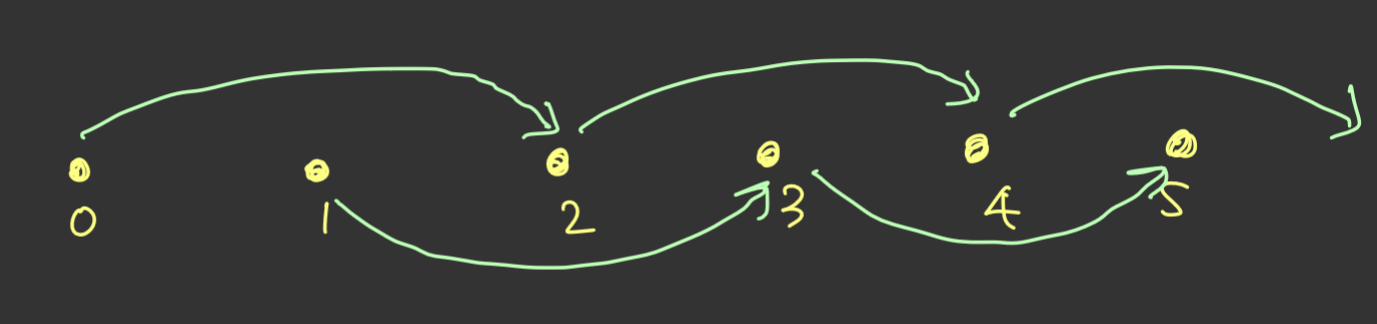
\includegraphics[width=0.7\linewidth]{leapfrog}
	\caption{Leap-frog}\label{fig:leapFrog}
\end{figure}

\subsubsection{Robert-Asselin Filter}
After solving for $\ve y_{n+1}$, we apply a time filter to $\ve y_n$ to ``smooth'' out the scheme. Define \[\ve y_n^{\text{new}}=\ve y_n+\frac\nu2(\ve y_{n-1}-2\ve y_n+\ve y_{n+1}),\] where $0.01\leq \nu\leq 0.2$ is a smoothing parameter. This adds a small fraction of the two outer points to $\ve y_n$. We then set $\ve y_{n+1}$ to be $\ve y_n^\text{new}$ and $\ve y_{n+1}$ to be $\ve y_n$ before taking the next time step.

\subsection{Other methods}
We introduce a few more second order schemes.
\subsubsection{Mid-point}
Explicit mid-point takes a half forward Euler step before performing the full step
\[\ve y_{n+1}=\ve y_n + \ve f\Paren{\ve y_n+f(\ve y_n,t_n)\frac{\dt}2,t_{n+\frac12}}\dt.\]

Implicit mid-point is \[y_{n+1}	=y_n+f\Paren{\frac{y_n+y_{n+1}}{2},t_{n+\frac12}}\dt.\]
\subsubsection{Trapezoidal}
The trapezoidal method (also called Crank-Nicolson) is a combination of forward and backward Euler \[y_{n+1}=y_n+\Paren{\frac{f(y_n,t_n)+f(y_{n+1},t_{n+1})}{2}}\dt.\]

\begin{eg}
Consider the ODE $\dder yt=-kt$ with $y(t_0)=1$. The explicit mid-point gives \[y_1=-k\dt+\frac{k}{2}(\dt)^2.\] Since the ODE is linear, the trapezoidal method is equivalent to implicit mid-point \[y_1=\frac{1-\frac k2\dt}{1+\frac k2\dt}.\]
\end{eg}

\subsection{Multi-step}
The typical family of multi-step methods are the Adams-Bashforth methods. These are explicit. The key idea is to fit a polynomial to $f(t)$ and integrate over the $t$-step.
\subsubsection{AB2}
For convenience, set $t=0$ at $y_n$. Then \[y_{n+1}=y_n+\int_0^{\dt} f(y_n,t)\dd t\]
 We use the points at $n$ and $n+1$ to fit a linear polynomial to $f_n$, i.e. $f(t)=at+b$. At $t=0$, $f_n=b$ and at $t=-\dt$, $f_{n-1}=-a\dt+b$. It follows that $b=f_n$ and $a=\frac{f_n-f_{n-1}}{\dt}$. Thus, \[y_{n+1}=y_n+\int_0^{\dt}(at+b)\dd t=y_n+\Paren{\frac{a}2(\dt)^2+b\dt}=y_n+\Paren{\frac32f_n-\frac12f_{n-1}}\dt.\]
 This defines the second order Adams-Bashforth method.
\subsubsection{AB3}
Similarly, fitting a second order $f(t)=at^2+bt+c$ at times $t\in\set{0,-\dt,-2\dt}$ yields \[c=f_n,\quad a=\frac{f_{n-2}-2f_{n-1}+f_n}{2(\dt)^2}, \quad b=\frac{f_{n-2}-4f_{n-1}+3f_n}{2\dt}.\] By integrating, we arrive at \[y_{n+1}=y_n+\Paren{\frac5{12}f_{n-2}-\frac{16}{12}f_{n-1}+\frac{23}{12}f_n}\dt.\]
Higher order methods can be derived in a similar way. Note that AB1 is forward Euler. If we use $f_{n+1}$ instead of $f_{n-1}$, we get the family of implicit Adams-Moulton methods (of which backward Euler is a member of).
\begin{ex}
	Show that the coefficients of $f_i$ in an Adams-Bashforth method always sum to 1.
\end{ex}

\subsection{Numerical stability}
Consider the differential equation $\dder yt=-\lambda y$ (for $\lambda>0$) with initial condition $y(0)=y_0$. The exact solution is $y=y_0e^{-\lambda t}$. We say that a scheme is \emph{numerically stable} if $y_n\to 0$ as $n\to \infty$.

For forward Euler, \[y_{n}=(1-\lambda \dt)y_n =(1-\lambda \dt)^ny_0.\] Thus, if $|1-\lambda \dt|>1$, $y_n$ grows and thus is unstable. So we need $\dt\leq\frac2\lambda$ for stability. 

For backward Euler, \[y_n=\frac{y_n}{1+\lambda \dt}=\Paren{\frac{1}{1+\lambda\dt}}^ny_0.\] Since $\frac{1}{1+\lambda\dt}<1$ for all $\dt>0$, backward Euler is unconditionally stable. Similarly, implicit midpoint is also unconditionally stable as \[y_n=\Paren{\frac{1-\frac\lambda2\dt}{1+\frac\lambda2\dt}}^ny_n.\]

\section{Partial differential equations}
	A general linear second order PDE in two variables is given by \[a\pder\phi{x_1}+b\frac{\partial^2\phi}{\partial x_1\partial x_2}+c\pder\phi{x_2}+d\der\phi{x_1}+e\der\phi{x_2}+f\phi = g.\]
The discriminant is \[\Delta = b^2-4ac \implies \begin{cases}
	\Delta<0 & \text{elliptic},\\ \Delta =0& \text{parabolic}, \\\Delta>0 &\text{hyperbolic}.
\end{cases}\]
In general, \[\sum_{ij}A_{ij}\frac{\partial^2\phi}{\partial x_i\partial x_j}+\sum_i B_i\der\phi{x_i}+C\phi = D.\]

This PDE is called \emph{elliptic} if none of the eigenvalues vanish and all have the same sign; \emph{parabolic} if ne eigenvalue vanishes and the remainder have the same sign; \emph{hyperbolic} if none of the eigenvalues vanish and one has the opposite sign.

\subsection{Parabolic PDEs}

Consider the diffusion equation with diffusivity $\kappa>0$ \[\der\phi t=\kappa\pder\phi x.\] This is a parabolic second order PDE. 

Diffusing equations have causality, i.e. the direction of time matters. Information spreads on scales $\delta\sim\sqrt{\kappa t}$ as in Figure~\ref{fig:diffusionTopHat} - the time step cannot be larger, otherwise the scheme becomes unstable.

\begin{figure}
	\centering
	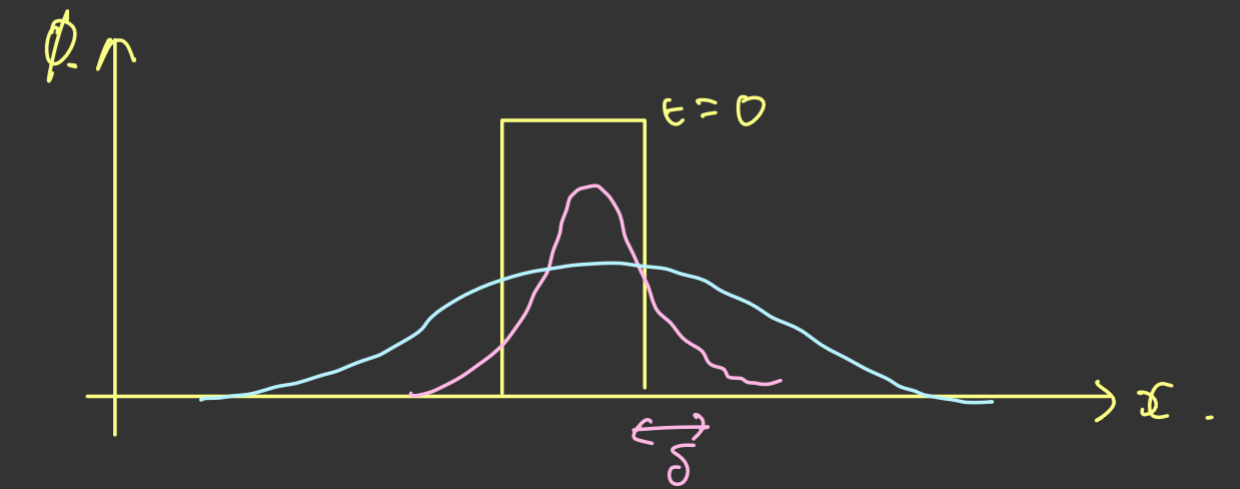
\includegraphics[width=0.7\textwidth]{diffusionSpreading}
	\caption{Diffusion spreading}
	\label{fig:diffusionTopHat}
\end{figure}

\begin{eg}
	Consider diffusion equation on $0\leq x\leq L$ and $0\leq t\leq T$.  Let $\phi_j^n=\phi(x_j,t_n)$ where $t_n=n\dt$ and $x_j=j\dx$. The domain is discretised in Figure~\ref{fig:diffusionDiscret}.
	
	\begin{figure}\centering
		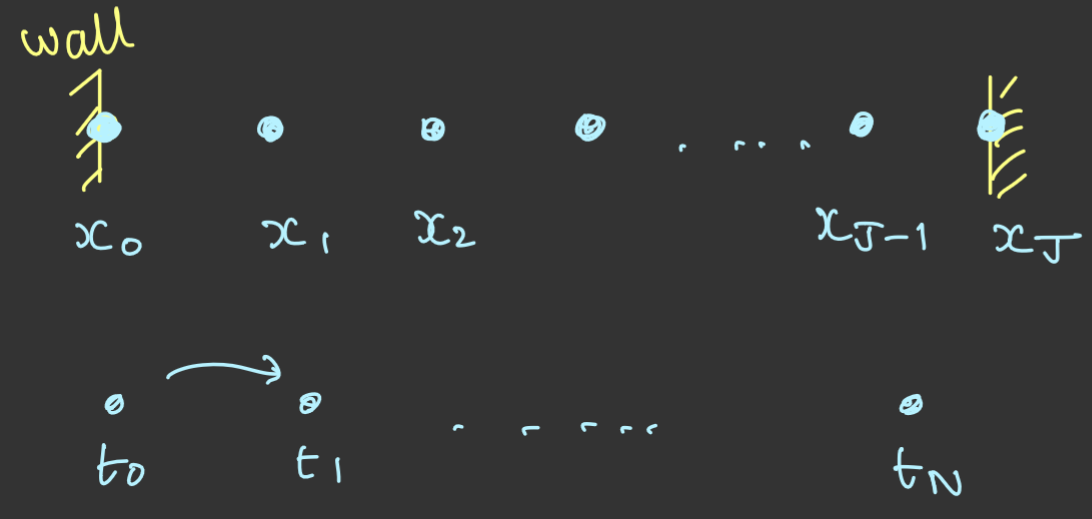
\includegraphics[width=0.7\textwidth]{discretisingDiffusion}
		\caption{Discretising the diffusion equation domain}\label{fig:diffusionDiscret}
	\end{figure}
	
	Using forward Euler, \[\frac{\phi_j^{n+1}-\phi_j^n}{\dt}=\kappa\frac{\phi_{j+1}^n-2\phi_j^n+\phi^n_{j-1}}{(\dx)^2}.\] It follows that \[\phi_j^{n+1}=\phi_j^n+\frac{\kappa\dt}{(\dx)^2}\Paren{\phi_{j+1}^n-2\phi_n^n+\phi_{j-1}^n}.\] This is straightforward to solve as forward Euler explicit. On the other hand, implicit backward Euler is \[\frac{\phi_j^{n+1}-\phi_j^n}{\dt}=\kappa\frac{\phi_{j+1}^{n+1}-2\phi_j^{n+1}+\phi^{n+1}_{j-1}}{(\dx)^2}.\] There are three unknowns, so we can not solve this directly. We solve this in Section~\ref{sec:elliptic}.

\end{eg}

\subsection{Boundary conditions}
A Dirichlet boundary condition is when we specify $\phi$ on solid boundaries. For example, $\phi(0,t)=1$ or $\phi(L,t)=0.5\sin(2\pi t)$.

Neumann boundary conditions specify the normal derivative. For example, $\der\phi x(0,t)=0$ (no flux), $\der\phi x(L,t)=F$ (specified flux).

We can mix the boundary conditions (Robin boundary conditions) to get $a\phi+b\der\phi x=c$.

Dirichlet boundary conditions are easy to implement by setting $\phi$ at the boundary. Neumann boundary conditions are a bit more complicated. We can use a 1-sided derivative with a grid point on the boundary: \[\der\phi x(0,t)=0\implies \frac{\phi_1^n-\phi_0^n}{\dx}=0\implies \phi_0^n=\phi_1^n.\] This is only first order accurate. A better place for the boundary is between two midpoints, which results in a second order accurate centred derivative. This can be implemented in two ways. The first is using ``ghost points'', i.e. put $\phi_0$ outside the domain. This may not be appropriate for complicated domains. The second way is to absorb the boundary conditions into the finite difference operator. For example, if $\kappa \der\phi x\eval{0.5}^n=0$, \[\kappa \pder\phi x\Eval1^n=\der{}x\Paren{\kappa\der\phi x}\Eval 1^n=\frac{\kappa\der\phi x\eval{1.5}^n-\kappa \der\phi x\eval{0.5}^n}{\dx}=\frac{\kappa}{\dx}(\phi_2^n-\phi_1^n).\]


\subsection{Hyperbolic PDEs}
Consider the wave equation \[\ddder\phi t = c^2 \ddder\phi x.  \] This is a hyperbolic PDE. Factoring, \begin{equation}\label{eq:waveRe}\Paren{\der{}t + c\der{}x}\Paren{\der{}{t}-c\der{}x}\phi = 0.\end{equation} Let $p=x+ct$ and $q=x-ct$, then $x=\frac{p+q}2$ and $t=\frac{p-q}{2c}$. From the chain rule, it follows that \begin{align*}\der\phi p&=\der\phi x\der xp+\der\phi t\der tp=\frac12\der\phi x+\frac1{2c}\der\phi t\\\der\phi q&=\der\phi x\der xq+\der\phi t\der tq=...\end{align*}
...
Substituting into Equation~\ref{eq:waveRe}, we get the hyperbolic PDE \[\der{^2\phi}{p\partial q}=0.\]
Integrating with respect to $p$ and $q$, \[\der\phi q=f'(q) \implies \phi = f(q)+g(p),\] for some choice of $f$ and $g$. Thus $\phi(x, t)=f(x,t)+g(x,t)...$. We see that $\phi$ is constant along lines of $x-ct$ and $...$ as in Figure~\ref{fig:waveMove}.

\begin{figure}\centering
	\includegraphics[width=0.7\textwidth]{example-image-golden}
	\caption{Wave}\label{fig:waveMove}
\end{figure}

\begin{eg}
	Consider the wave equation on $0\leq t\leq \infty$ and $0\leq x\leq L$. At time $t=0$, since we have a second derivative in time, we need two initial conditions (corresponding to $f$ and $g$). We need one boundary condition each on $x=0$ (corresponding to $f$) and $x=L$ (corresponding to $g$). This is illustrated in Figure~\ref{fig:waveDomain}. For example, we could take boundary conditions $\phi(x,0)$, $\der{}t\phi(x,0)$, $\phi(0,t)$ and $\phi(L,t)$.
	
	\begin{figure}\centering
		\includegraphics[width=0.7\textwidth]{example-image-golden}
		\caption{Wave domain discretise}\label{fig:waveDomain}
	\end{figure}
	
	 Adding an advection term complicates things. One way to treat advection is to use sponge layers.
	 
	 To solve the wave equation, we may use a centred difference for both second derivatives \[U_j^{n+1}-2U_j^n+U_j^{n-1}{(\dt)^2}=c^2\Paren{\frac{U^n_{j+1}-2U_j^n+U^n_{j-1}}{\dx^2}},\] where $U_j^n = \phi(x_jt_n)$ This is second order in both time and space. For stability, we need $\size{\dx}<\size{c\dt}$, i.e. the wave shouldn't travel more than one grid space in one time step.
	
\end{eg}
\subsection{Advection equations}
An advection equation has the form \[\der\phi t+u\der\phi x=0.\] This models a fluid parcel moving at velocity $u>0$ while maintaining its $\phi$. If $u$ is constant, then $\phi(x,t)=f(x-uy)$.

Using forward Euler, we get the ``upwind'' scheme \[\frac{\phi_j^{n+1}-\phi_j^n}{\dt}+u\Paren{\frac{\phi^n_j-\phi^n_{j-1}}{\dx}}=0.\] This is illustrated in Figure~\ref{fig:advectionEuler}. This is unstable if $u<0$ or $u>\frac{\dx}{\dt}$ and is called the Courant–Friedrichs–Lewy (CFL) condition. If $u<0$, swap the direction of the discretisation.

	\begin{figure}\centering
	\includegraphics[width=0.7\textwidth]{example-image-golden}
	\caption{Advection Euler grid}\label{fig:advectionEuler}
	\end{figure}
	
More generally, \[\phi_j^{n+1}=\phi_j^n-\begin{cases}
	\frac{u\dt}{\dx}(\phi_j^n-\phi_{j-1}^n)&\text{if }u\geq0,\\\frac{u\dt}{\dx}(\phi_{j+1}^n-\phi_j^n)&\text{if }u<0.
\end{cases}\] This is the general ``upwind'' scheme and is first order in space and time.

To get higher order in time, we can use an AB scheme. For second order space, we can try using a centred difference 
\[\frac{\phi_j^{n+1}-\phi_j^n}{\dt}+u\Paren{\frac{\phi^n_{j+1}-\phi^n_{j-1}}{2\dx}}=0.\] But this is an unstable scheme. However, the Lax-Friedrichs scheme works (and is stable) by adding diffusion in time \[\frac{\phi_j^{n+1}-\frac12(\phi_{j+1}^n+\phi_{j-1}^n)}{\dt}+{\frac{u(\phi^n_{j+1}-\phi^n_{j-1})}{2\dx}}=0.\]


\subsubsection{Diffusive errors}

Consider the upwind scheme\[\phi_{j-1}^n=\phi_j^n-\der\phi x\Eval j^n\dx+\pder\phi x\Eval j^n\frac{(\dx)^2}2+O((\dx)^3).\] Then \[\frac{\phi_j^{n+1}-\phi_j^n}\dt=-u\Paren{\frac{\phi_j^n-\phi_{j-1}^n}{\dx}}=-u\der\phi x\Eval j^n + \frac{u\dx}2\pder\phi x\Eval j^n + O((\dx)^2).\] The coefficient $\frac{u\dx}2$ is the effective diffusivity.

\subsubsection{Dispersive errors}

Consider centred advection. Using the Taylor expansion, \[\phi_{j\pm 1}^n=\phi_j^n\pm \der\phi x\Eval j^n\dx+\pder\phi x\Eval j^n\frac{(\dx)^2}2\pm \pder[3]\phi x\Eval j^n\frac{(\dx)^3}6+O((\dx)^4),\]
we get \[u\der\phi x \approx u\Paren{\frac{\phi_{j+1}^n-\phi_{j-1}^n}{2\dx}}=u\der\phi x\Eval j^n+\frac{u(\dx)^2}6\pder[3]\phi x\Eval j^n.\]

Take the solution $\phi=\phi_0\exp(i(kx-wt))$. Pure advection becomes \[\der\phi t+u\der\phi x=-\implies -i\omega+iku =0\implies \frac\omega k = \dder\omega k=u.\]

Numerically, \[\der\phi t+ u\der \phi x+\frac{u(\dx)^2}6\pder[3]\phi x=0\implies -i\omega+iku-ik^3\frac{u(\dx)^2}{6}=0\]
Then \[\frac{\omega}k=u-\frac{u(\dx)^2}{6}k^2,\quad \dder\omega k= u +...\]
\section{Von Neumann analysis}


\section{Numerical linear algebra}\label{sec:numla}


\appendix
\section{Background theory}
\subsection{\texorpdfstring{Big $O$}{Big O} notation}\label{sec:bigO}
\subsection{Taylor expansions}\label{sec:taylor}
\begin{thm}[Taylor]\label{thm:taylor}
	\[f(x)=f(x_0)+f'(x_0)(x-x_0) + \cdots\]
\end{thm}

\nocite{*}
\bibliographystyle{abbrv}
\bibliography{refs}
\addcontentsline{toc}{section}{References}

\label{lastpage}
\end{document}
